\chapter{crate与模块}\label{ch08}

\emph{This is one note in a Rust theme: systems programmers can have nice things.}

\begin{flushright}
    ——Robert O'Callahan, “\href{https://robert.ocallahan.org/2016/08/random-thoughts-on-rust-cratesio-and.html}{Random Thoughts on Rust: crates.io and IDEs}”
\end{flushright}

假设你在编写一个仿真蕨类植物从细胞开始生长的程序。你的程序就像蕨类一样,一开始非常简单,可能所有代码都在单个文件里——就像一个孢子。随着它逐渐成长,它开始逐渐建立起内部的结构,不同的片段负责不同的功能。它将分裂为多个文件,可能覆盖整个目录树。随着时间的推移,它可能会成为整个软件生态系统的重要组成部分 。对于任何成长到不仅仅是几个数据结构和几百行代码的程序,都必须要对代码进行组织。

这一章将会介绍Rust中用于组织程序的特性:crate和模块。我们还会介绍Rust crate的结构和分发相关的话题,包括如何编写文档和测试Rust代码,如何禁用不需要的编译器警告,如何使用Cargo来管理项目依赖和版本,如何在Rust的公开crate仓库:crates.io上发布开源的库,crate的版本如何演变,等等。我们将使用蕨类仿真程序作为我们的例子。

\section{Crate}

Rust程序由\emph{crates}组成。每一个crate都是一个完整的、一体的单元:一个库或可执行文件的所有代码、加上相关的测试、示例、工具、配置、以及一些其他东西。为了编写你自己的蕨类模拟器,你可能需要使用和3D图形、生物信息学、并行计算等相关的第三方库。这些库就像箱子一样(见\hyperref[f8-1]{图8-1})。

\begin{figure}[htbp]
    \centering
    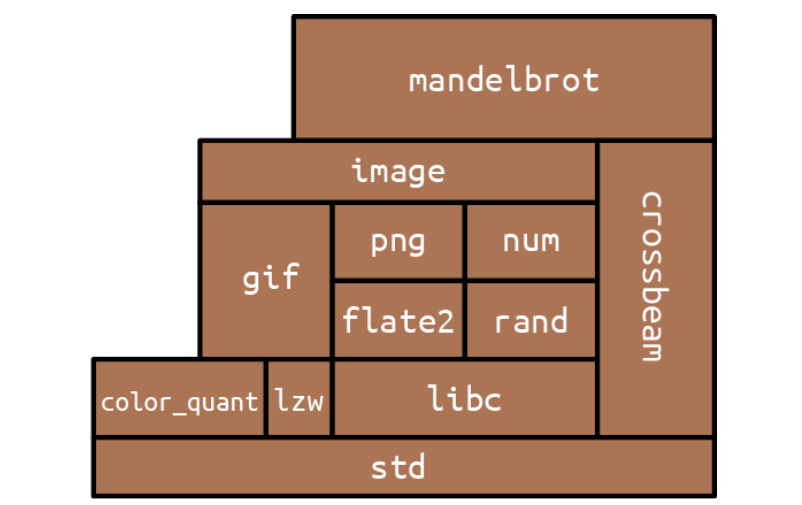
\includegraphics[width=0.9\textwidth]{../img/f8-1.png}
    \caption{一个crate和它的依赖}
    \label{f8-1}
\end{figure}

查看crate是什么以及它们是如何工作的最简单方法就是使用带有\texttt{--verbose}参数的\texttt{cargo build}来构建一个有一些依赖的程序。我们用“\hyperref[mandelbrot]{一个并发的曼德勃罗集}”作为示例。结果如下所示:
\begin{minted}{text}
    $ cd mandelbrot
    $ cargo clean   # delete previously compiled code
    $ cargo build --verbose
        Updating registry `https://github.com/rust-lang/crates.io-index`
     Downloading autocfg v1.0.0
     Downloading semver-parser v0.7.0
     Downloading gif v0.9.0
     Downloading png v0.7.0
    
    ... (downloading and compiling many more crates)

        Compiling jpeg-decoder v0.1.18
          Running `rustc
             --crate-name jpeg_decoder
             --crate-type lib
             ...
             --extern byteorder=.../libbyteorder-29efdd0b59c6f920.rmeta
             ...
        Compiling image v0.13.0
          Running `rustc
             --crate--name image
             --crate-type lib
             ...
             --extern byteorder=.../libbyteorder-29efdd0b59c6f920.rmeta
             --extern gif=.../libgif-a7006d35f1b58972.rmeta
             --extern jpeg_decoder=.../libjped_decoder-5c10558d0d57d300.rmeta
        Compiling mandelbrot v0.1.0 (/tmp/rustbook-test-files/mandelbrot)
          Running `rustc
             --edition=2018
             --crate-name mandelbrot
             --crate-type bin
             ...
             --extern crossbeam=.../libcrossbeam-f87b4b3d3284acc2.rlib
             --extern image=.../libimage-b5737c12bd641c43.rlib
             --extern num=.../libnum-1974e9a1dc582ba7.rlib -C link-arg=-fuse-ld=lld`
         Finished dev [unoptimized + debuginfo] target(s) in 16.94s
\end{minted}

我们重新格式化了\texttt{rustc}的命令行来改善可读性,并且删掉了很多和我们的讨论无关的编译器选项,用省略号(\ldots)代替了它们。

你可能还记得,当我们完成曼德勃罗集程序时,它的\texttt{main.rs}包含几个引入其它crate的\texttt{use}声明:
\begin{minted}{Rust}
    use num::Complex;
    // ...
    use image::ColorType;
    use image::png::PNGEncoder;
\end{minted}

哦我们还在\texttt{Cargo.toml}中指定了每个crate的版本:
\begin{minted}{toml}
    [dependencies]
    num = "0.4"
    image = "0.13"
    crossbeam = "0.8"
\end{minted}

这里的\emph{依赖}指这个程序使用的其它crate,也就是我们依赖的代码。我们可以在\href{https://crates.io}{crates.io}中找到这些crate,那是Rust社区用于存放开源的crate的网站。例如,我们可以访问crates.io并搜索图片库来找到\texttt{image}库。crates.io上的每个crate的页面上会显示它的\texttt{README.md}文件和到文档和源代码的链接,还有一行配置例如\texttt{image = "0.13"},你可以复制这一行并添加到你的\texttt{Crago.toml}中。这里显示的版本号直接用了我们在编写这个程序时这三个包的最新版本。

Cargo的输出说明了这些信息是如何被使用的。当我们运行\texttt{cargo build}时,Cargo会首先从crates.io下载这些crate的指定版本的源码。然后,它读取那些crate的\texttt{Cargo.toml}文件,下载\emph{它们}的依赖,然后递归操作。例如,\texttt{image} crate的0.13.0版本的源代码中包含一个\texttt{Cargo.toml}文件,内容如下:
\begin{minted}{toml}
    [dependencies]
    byteorder = "1.0.0"
    num-iter = "0.1.32"
    num-rational = "0.1.32"
    num-traits = "0.1.32"
    enum_primitive = "0.1.0"
\end{minted}

看到这些内容,Cargo知道在它可以使用\texttt{image}之前,它必须先拉取这些crate。我们称它们为\texttt{mandelbrot}的\emph{间接(transitive)}依赖。所有这些依赖的集合告诉了Cargo需要知道的有关如何构建和构建顺序的一切信息,它被称为crate的\emph{依赖图}。Cargo自动处理依赖图和间接依赖的能力是程序员们付出时间和努力的一大胜利。

当获得了源代码之后,Cargo会编译所有的crate。它会运行Rust的编译器\texttt{rustc},一次编译依赖图中的一个crate。当编译这些库时,Cargo会使用\texttt{--crate-type lib}选项。这告诉\texttt{rustc}不要寻找\texttt{main()}函数,而是产生一个包含编译过代码的\texttt{.rlib}文件,这个文件可以被用于创建可执行文件和其他\texttt{.rlib}文件。

当编译程序时,Cargo会使用\texttt{--crate-type bin},编译的结果将是一个目标平台的二进制可执行文件:例如在Windows上就是\texttt{mandelbrot.exe}。

对于每一个\texttt{rustc}命令,Cargo都会传递\texttt{--extern}选项,给出crate用到的每一个库的名称。这样,当\texttt{rustc}看到一行类似于\texttt{use image::png::PNGEncoder}的代码时,它可以分辨出\texttt{image}是另一个crate的名字,而且Cargo传递的选项让它知道该从哪里寻找编译好的crate。Rust的编译器需要访问这些\texttt{.rlib}文件,因为它们包含编译好的库中的代码。Rust将会将代码静态链接到最终的可执行文件中。\texttt{.rlib}还包含类型信息,因此Rust可以通过检查确保我们在代码中使用的库的特性确实存在而且被正确使用。它还包含一份crate的public内联函数、泛型、宏、特性的拷贝,这些东西只有当Rust看到我们如何使用它们时才可以将它们编译为机器代码。

\texttt{cargo build}支持各种选项,其中的大部分都超出了本书的范围,不过我们在这里会提到其中一个:\texttt{cargo build --release}会生成优化后的构建。Release构建运行得更快,但需要更长的时间来编译,而且它们不检查整数溢出、跳过\texttt{debug\_assert!()}断言,并且它们在panic生成的堆栈追踪通常不太可靠。

\subsection{版本}

Rust有极强的兼容性保证。任何在Rust 1.0中能编译的代码必须在Rust 1.50或者1.900(如果发布了的话)中也能编译。


但有时社区会遇到一些令人信服的扩展语言的建议,这可能会导致旧代码不能再编译。例如,经过了多次讨论之后,Rust确定了一种支持异步编程的语法,将标识符\texttt{async}和\texttt{await}重新用作关键字(见\hyperref[ch20]{第20章})。但这项语言的改变可能会导致使用\texttt{async}或者\texttt{await}作为变量名的代码不能再编译。

为了在不破坏这些现有代码的前提下演变,Rust使用了\emph{版本}。Rust的2015版本和Rust 1.0兼容。2018版本将\texttt{async}和\texttt{await}改为关键字、精简了模块系统、还引入了一些和2015版本不兼容的其它语言更改。每个crate在\texttt{Cargo.toml}文件中的\texttt{package}节中用一行类似如下的说明指定Rust的版本:
\begin{minted}{Rust}
    edition = "2018"
\end{minted}

如果缺少这个关键字,将会假设使用2015版本,因此旧的crate完全不需要做任何更改。但如果你想使用异步函数或者新的模块系统,你需要确保\texttt{Cargo.toml}中有\texttt{edition = "2018"}(或者可能更新的版本)。

Rust保证编译器将总是接受语言的所有版本,并且程序可以自由混合使用不同版本编写的crate。即使一个2015版本的crate依赖一个2018版本的crate也没有问题。换句话说,一个crate的版本只影响它的代码是如何被构建的,版本的区别只体现在代码编译的时候。这意味着没有必要更新旧的版本来适配现代Rust的生态。类似的,也没有必要将crate保持在旧版本来避免影响到它的用户。你只需要在想使用新的语言特性时更改自己代码中的版本。

版本并不是每年都会更新,只有当Rust项目觉得有必要出新版本的时候才会更新。例如,没有2020版本。把\texttt{edition}设置为\texttt{"2020"}将会导致错误。\href{https://doc.rust-lang.org/stable/edition-guide}{Rust版本指南}介绍了每一个版本中的变化,并提供了版本系统的背景知识。

使用最新版本几乎总是一个好主意,尤其是新编写代码时。\texttt{cargo new}会默认创建最新版本的项目。这本书中将始终使用2018版本。

如果你有一个用更旧版本的Rust编写的crate,\texttt{cargo fix}命令也许可以帮你自动把代码更新到更新的版本。Rust版本指南详细解释了\texttt{cargo fix}命令。

\subsection{构建配置}
有几个\texttt{Cargo.toml}中的配置选项可以影响到\texttt{cargo}生成的\texttt{rustc}命令行(\hyperref[t8-1]{表8-1})。

\begin{table}[htbp]
    \caption{Cargo.toml配置节}
    \centering
    \begin{tabular}{ll}
        \hline
        \textbf{命令行}     & \texttt{使用到的Cargo.toml节}   \\
        \hline
        \texttt{cargo build} & \texttt{[profile.dev]}   \\
        \rowcolor{tablecolor}
        \texttt{cargo build --release} & \texttt{[profile.release]} \\
        \texttt{cargo test}  & \texttt{[profile.test]}  \\
    \end{tabular}
\end{table}

通常默认的行为就足够了,但我们会发现一个例外是你想使用一个profiler——一个用于测量程序使用CPU时间情况的工具。为了从profiler获取最准确的数据,你将同时需要优化(通常只在release构建中可用)和调试符号(通常只在debug构建中可用)。为了同时启用两者,在\texttt{Cargo.toml}中添加:
\begin{minted}{toml}
    [profile.release]
    debug = true    # 允许在release构建中启用调试符号
\end{minted}

\texttt{debug}设置控制是否给\texttt{rustc}传递\texttt{-g}选项。有了这个配置,当你输入\texttt{cargo build --release}时,你将会得到一个带有调试符号的二进制文件。优化的设置将不会被影响。

\hyperref[https://doc.rust-lang.org/cargo/reference/manifest.html]{Cargo文档}中列出了很多其他你可以在\texttt{Cargo.toml}中调整的设置。

\section{模块}

如果说crate决定了项目之间的代码共享,那么\emph{模块}则决定了项目\emph{内部}的代码组织。它们扮演了Rust中的命名空间——一种包含函数、类型、常量等内容的容器,这些模块组成了你的Rust程序或库。一个模块看起来类似于这样:

\begin{minted}{Rust}
    mod spores {
        use cells::{Cell, Gene};

        /// 成熟蕨类植物产生的细胞。它会随着风飘散,
        /// 这也是蕨类生命周期的一部分。一个孢子会成长为一个原叶体——
        /// 一个宽达5mm的完整的独立有机体。它会产生受精卵,
        /// 这些受精卵会成长为新的蕨类植物(植物的性别很复杂)。
        pub struct Spore {
            ...
        }

        /// 模拟通过减数分裂产生孢子的过程。
        pub fn produce_spore(factory: &mut Sporangium) -> Spore {
            ...
        }

        // 提取一个孢子中的基因。
        pub(crate) fn genes(spore: &Spore) -> Vec<Gene> {
            ...
        }

        /// 混合基因为减数分裂做准备(分裂间期的一部分)。
        fn recombine(parent: &mut Cell) {
            ...
        }

        ...
    }
\end{minted}

一个模块是\emph{item}的集合,\texttt{item}是命名的特性例如例子中的\texttt{Spore}结构体和两个函数。\texttt{pub}关键字将item设为公有的,因此可以从模块外边访问。

一个函数被标记为\texttt{pub(crate)},意味着它在这个crate中任何地方都可以访问,但不作为外部接口的一部分公开。它不能被其他crate使用,也不会在crate的文档中显示。

任何没有被标记为\texttt{pub}的都是私有的,只能在定义它的模块和子模块中使用:
\begin{minted}{Rust}
    let s = spores::produce_spore(&mut factory);    // ok
    
    spores::recombine(&mut cell);   // 错误:`recombine`是私有的
\end{minted}

将item标记为\emph{pub}通常称为“导出”这个item。

这一节的剩余部分将覆盖使用模块所需要了解的细节:
\begin{itemize}
    \item 我们会展示如果需要的话怎么嵌套模块和把它们分布在不同的文件和目录中。
    \item 我们会解释Rust从其他模块中引用item的路径语法,并展示怎么导入item,这样就不需要每次都写出完整的路径。
    \item 我们会接触Rust对结构体字段的细粒度控制。
    \item 我们会介绍\emph{prelude}模块,它通过收集几乎所有用户都会用到的常见导入来减少重复的导入。
    \item 我们会展示\emph{常量}和\emph{静态量},这是两种为了清晰和一致性而设计的定义命名变量的方式。
\end{itemize}

\subsection{嵌套模块}

模块可以嵌套,事实上一个模块只是一些子模块的集合的情况是很常见的:
\begin{minted}{Rust}
    mod plant_structures {
        pub mod roots {
            ...
        }
        pub mod stems {
            ...
        }
        pub mod leaves {
            ...
        }
    }
\end{minted}

如果你想要让嵌套模块中的一个item对其他crate可见,那需要保证将它\emph{和所有嵌套包含它的模块}标记为public。否则你会看到一个类似这样的警告:
\begin{minted}{text}
    warning: function is never used: `is_square`
      --> src/crates_unused_items.rs:23:9
       |
    23 | /         pub fn is_square(root: &Root) -> bool {
    24 | |             root.cross_section_shape().is_square()
    25 | |         }
       | |_________^
       |
\end{minted}

可能这个函数这时确实是死代码。但如果你是想将它用在其他crate中,Rust会让你明白它实际上并不可见。你需要保证嵌套包含它的模块也都被标记为\texttt{pub}。

也可以声明\texttt{pub(super)},让一个item只在父模块中可见。\texttt{pub(in <path>)}可以让它在一个指定的父模块和其后代中可见。这在深层嵌套的模块中很有用:
\begin{minted}{Rust}
    mod plant_structures {
        pub mod roots {
            pub mod products {
                pub(in crate::plant_structures::roots) struct Cytokinin {
                    ...
                }
            }

            use products::Cytokinin;    // ok: 在`roots`模块中
        }

        use roots::products::Cytokinin; // error: `Cytokinin`是私有的
    }

    // error: `Cytokinin`是私有的
    use plant_structures::roots::products::Cytokinin;
\end{minted}

通过这种方式,我们可以写出一个有数量庞大的代码和完整的模块层次结构的程序,不管这些模块的关系如何,我们都可以将整个程序写在单个文件里。

但实际上以这种方式来工作非常的痛苦,因此还有另一种方案。

\subsection{单独文件中的模块}
一个模块还可以这么写:
\begin{minted}{Rust}
    mod spores;
\end{minted}

之前,我们还在花括号中包含了\texttt{spores}模块的主体。这里,我们通过这种方式告诉Rust编译器\texttt{spores}模块在一个单独的叫\texttt{spores.rs}的文件里:
\begin{minted}{Rust}
    // spores.rs

    /// 成熟蕨类植物产生的一个细胞...
    pub struct Spore {
        ...
    }

    /// 模拟减数分裂产生孢子的过程。
    pub fn produce_spore(factory: &mut Sporangium) -> Spore {
        ...
    }

    /// 从一个孢子中提取基因。
    pub(crate) fn genes(spore: &Spore) -> Vec<Gene> {
        ...
    }

    /// 混合基因为减数分裂做准备(分裂间期的一部分)。
    fn recombine(parent: &mut Cell) {
        ...
    }
\end{minted}

\texttt{spores.rs}只包含组成模块的item。它并不需要任何说明来表明它是一个模块。

这个\texttt{spores}模块和我们在上一节中展示的版本的\emph{唯一}不同就是代码的位置。有关公有性和私有性的规则和之前完全相同。Rust从来不会单独编译模块,即使它们在单独的文件里。当你构建一个Rust的crate的时候,你总是要重新编译它里面所有的模块。

一个模块也可以有自己的目录。当Rust看到\texttt{mod spores;}时,它会检查\texttt{spores.rs}和\texttt{spores/mod.rs},如果这两个文件都不存在或者都存在就会报错。这个例子中我们使用了\texttt{spores.rs},因为\texttt{spores}模块没有任何子模块。但考虑一下我们之前写的\texttt{plant\_structures}模块。如果我们决定将那个模块和它的三个字模块分割在单独的文件中,最终的项目看起来就是这样:
\begin{minted}{text}
    fern_sim/
    |—— Cargo.toml
    |—— src/
        |—— main.rs
        |—— spores.rs
        |—— plant_structures/
            |—— mod.rs
            |—— leaves.rs
            |—— roots.rs
            |—— stems.rs
\end{minted}

在\texttt{main.rs}中,我们声明了\texttt{plant\_structures}模块:
\begin{minted}{Rust}
    pub mod plant_structures;
\end{minted}

这会导致Rust去加载\texttt{plant\_structures/mod.rs},这个文件里又声明了三个子模块:
\begin{minted}{Rust}
    // 在plant_structures/mod.rs中
    pub mod roots;
    pub mod stems;
    pub mod leaves;
\end{minted}

这三个模块的内容都被存储在单独的文件中,分别命名为\texttt{leaves.rs}、\texttt{roots.rs}、\texttt{stems.rs},和\texttt{mod.rs}一样在\texttt{plant\_structures}目录下。

使用同名的文件和目录来组成模块也是有可能的。例如,如果\texttt{stems}需要包含两个分别叫\texttt{xylem}和\texttt{phloem}的模块,我们可以选择将\texttt{stems}保留在\texttt{plant\_structures/stems.rs}中,然后添加一个新的\texttt{stems}目录:
\begin{minted}{Rust}
    fern_sim/
    |—— Cargo.toml
    |—— src/
        |—— main.rs
        |—— spores.rs
        |—— plant_structures/
            |—— mod.rs
            |—— leaves.rs
            |—— roots.rs
            |—— stems/
            |   |—— phloem.rs
            |   |—— xylem.rs
            |—— stems.rs
\end{minted}

然后在\texttt{stems.rs}中声明这两个新的子模块:
\begin{minted}{Rust}
    // 在plant_structures/stems.rs中
    pub mod xylem;
    pub mod phloem;
\end{minted}

这三种方式——模块在自己单独的文件中、模块在自己同名的目录中的\texttt{mod.rs}中,模块在自己单独的文件中并有一个同名的目录包含子模块——给了模块系统足够的灵活性来支撑你需要的任何程序结构。

\subsection{路径和导入}
\texttt{::}运算符用于访问模块中的特性。你的项目中任何地方的代码都可以通过路径来引用任何标准库的特性:
\begin{minted}{Rust}
    if s1 > s2 {
        std::mem::swap(&mut s1, &mut s2);
    }
\end{minted}

\texttt{std}是标准库的名称。路径\texttt{std}指向标准库的顶级模块。\texttt{std::mem}是在标准库中的一个子模块,\texttt{std::mem::swap}是\texttt{std::mem}模块中的一个public函数。

你可以始终用这方式编写所有的代码,每当你需要圆或字典时都写出\texttt{std::f64::consts::PI}和\texttt{std::collections::HashMap::new},但这样太过繁琐,而且难以阅读。替代方案是把一些特性\emph{导入}用到它们的模块:
\begin{minted}{Rust}
    use std::mem;

    if s1 > s2 {
        mem::swap(&mut s1, &mut s2);
    }
\end{minted}

\texttt{use}声明会导致\texttt{mem}变为\texttt{std::mem}在整个块或模块中的一个局部别名。

你也可以编写\texttt{std::mem::swap}来导入\texttt{swap}函数本身,而不是\texttt{mem}模块。然而,我们之前的方式被认为是最佳的风格:引入类型、trait和模块(例如\texttt{std::mem})然后使用相对路径访问函数、常量和其他成员。

可以依次导入若干个名字:
\begin{minted}{Rust}
    use std::collections::{HashMap, HashSet};   // 导入两个
    
    use std::fs::{self, File};  // 导入`std::fs`和`std::fs::File`
    
    use std::io::prelude::*;    // 导入所有内容
\end{minted}

这是写出所有单独导入的方式的缩写:
\begin{minted}{Rust}
    use std::collections::HashMap;
    use std::collections::HashSet;

    use std::fs;
    use std::fs::File;

    // std::io::prelude中的所有public item:
    use std::io::prelude::Read;
    use std::io::prelude::Write;
    use std::io::prelude::BufRead;
    use std::io::prelude::Seek;
\end{minted}

你可以使用\texttt{as}导入一个item并同时给它一个不同的局部名称:
\begin{minted}{Rust}
    use std::io::Result as IOResult;

    // 返回类型等价于`std::io::Result<()>`
    fn save_spore(spore: &Spore) -> IOResult<()>
    ...
\end{minted}

模块并不会\emph{自动}从父模块中继承名称。例如,假设我们的\texttt{proteins/mod.rs}有如下内容:
\begin{minted}{Rust}
    // proteins/mod.rs
    pub enum AminoAcid { ... }
    pub mod synthesis;
\end{minted}

那么\texttt{synthesis.rs}里的代码并不会自动导入类型\texttt{AminoAcid}:
\begin{minted}{Rust}
    // proteins/synthesis.rs
    pub fn synthesis(seq: &[AminoAcid]) // 错误:找不到类型`AminoAcid`
        ...
\end{minted}

每一个模块都会以空白的状态开始,必须导入它使用的名称:
\begin{minted}{Rust}
    // proteins/synthesis.rs
    use super::AminoAcid;   // 显式地从父模块中导入
    pub fn synthesize(seq: &[AminoAcid]) // ok
        ...
\end{minted}

默认情况下,路径是相对于当前模块的:
\begin{minted}{Rust}
    // 在proteins/mod.rs中

    // 从子模块中导入
    use synthesis::synthesize;
\end{minted}

\texttt{self}也是当前模块的同义词,因此我们可以写:
\begin{minted}{Rust}
    // 在proteins/mod.rs中

    // 导入一个枚举中的名字
    // 这样我们可以用`Lys`来表示赖氨酸,而不是`AminoAcid::Lys`
    use self::AminoAcid::*;
\end{minted}

或者简写为:
\begin{minted}{Rust}
    // 在proteins/mod.rs中

    use AminoAcid::*;
\end{minted}

(这里的\texttt{AminoAcid}的例子,有些违背我们之前提到的只导入类型、trait和模块的风格。如果我们的程序包含很长的氨基酸序列,那么根据奥威尔的第六原则:“Break any of these rules sooner than say anything outright barbarous.”(绝不要用粗俗语言,为此可以打破上面任一规则。)这么做也是有道理的。

路径中的\texttt{super}和\texttt{crate}关键字有特殊的含义:\texttt{super}指代父模块,\texttt{crate}指代包含当前模块的crate。

使用相对于crate根的路径而不是相对于当前模块的路径可以使在项目中移动代码变得更容易,因为这样的话计算当前模块的路径变了,导入也不会出错。例如,我们可以使用\texttt{crate}来写\texttt{synthesis.rs}:
\begin{minted}{Rust}
    // proteins/synthesis.rs
    use crate::proteins::AminoAcid; // 显式的相对于crate根的导入

    pub fn synthesize(seq: &[AminoAcid]) // ok
        ...
\end{minted}

子模块可以通过\texttt{use super::*}访问父模块中的私有item。

如果你有一个模块和当前正在使用的某一个模块同名,那么引用它们的时候就要小心了。例如,如果你的程序在\texttt{Cargo.toml}列出了\texttt{image} crate依赖,同时还有一个模块叫\texttt{image},那么以\texttt{image}开头的路径将会导致歧义:
\begin{minted}{Rust}
    mod image {
        pub struct Sampler {
            ...
        }
    }

    // 错误:这是指向`imaeg`模块,还是`image` crate?
    use image::Pixels;
\end{minted}

即使\texttt{image}模块没有\texttt{Pixels}类型,这个歧义也会被认为是错误:如果之后又添加了\texttt{Pixels}的定义,那么可能会改变路径指向的内容,这可能会令人迷惑。

为了解决歧义,Rust有一种特殊的路径称为\emph{绝对路径},它们以\texttt{::}开头,将总是指向一个外部的crate。为了指向\texttt{image} crate中的\texttt{Pixels}类型,你可以写:
\begin{minted}{Rust}
    use ::image::Pixels;    // `image` crate的`Pixels`
\end{minted}

为了指向你自己的模块中的`Sampler`类型,你可以写:
\begin{minted}{Rust}
    use self::image::Sampler;   // `image`模块的`Sampler`
\end{minted}

模块和文件的概念并不相同,但模块和Unix文件系统中的文件和目录存在自然的类比关系。\texttt{use}关键字创建别名,就像\texttt{ln}命令创建链接。路径类似于文件名,有绝对路径和相对路径两种形式。\texttt{self}和\texttt{super}类似于\texttt{.}和\texttt{..}这两个特殊的目录。

\subsection{标准prelude}
我们之前说每个模块都以“空白的状态”开始,但事实上并不是\emph{完全}空白的状态。

其中一点是,标准库\texttt{std}被自动链接到每个项目。这意味着你总是可以使用\texttt{std::whatever}这种方式来引用\texttt{std}里的item,例如\texttt{std::mem::swap()}。还有,一些特殊的常见名称,例如\texttt{Vec}和\texttt{Result}也被包含在\emph{标准prelude}中并且被自动导入。具体的行为就好像是包括跟模块在内的每个模块都以如下导入开始:
\begin{minted}{Rust}
    use std::prelude::v1::*;
\end{minted}

标注的prelude包含一些通用的trait和类型。

在\hyperref[ch02]{第2章}中时,我们提到了库有时会提供叫\texttt{prelude}的模块。但\texttt{std::prelude::v1}是唯一一个自动导入的。将一个模块命名为\texttt{prelude}只会一个约定,告诉用户他应该导入\texttt{*}。

\subsection{pub use声明}
即使\texttt{use}声明只是别名,它们也可以是公有的:
\begin{minted}{Rust}
    // in plant_structures/mod.rs
    ...
    pub use self::leaves::Leaf;
    pub use self::roots::Root;
\end{minted}

这意味着\texttt{Leaf}和\texttt{Root}是\texttt{plant\_structures}模块里的public item。它们实际上只是\texttt{plant\_structures::leaves::Leaf}和\texttt{plant\_structures::roots::Root}的别名。

标准的prelude就是以一系列\texttt{pub}导入的方式实现的。

\subsection{pub结构体字段}
一个模块可以包含用户用\texttt{struct}关键字定义的自定义结构体类型。我们将在\hyperref[ch09]{第9章}中介绍细节,但这是一个了解模块如何和结构体字段的可见性交互的好时机。

一个简单的结构体类似这样:
\begin{minted}{Rust}
    pub struct Fern {
        pub roots: RootSet,
        pub stems: StemSet
    }
\end{minted}

一个结构体的所有字段,包括私有字段,都可以在定义结构体的整个模块及其子模块中访问,在模块之外,只有公有的字段才可以被访问。

事实证明通过模块来实现访问控制,而不是像Java和C++那样通过类来实现,对于程序设计将是很大的帮助。不仅能减少重复“getter”和“setter”方法,还能消除类似C++中\texttt{friend}声明的需求。一个模块可以定义几个紧密结合的类型,例如\texttt{frond::LeafMap}和\texttt{frond::LeafMapIter},让它们能按需互相访问彼此的私有字段,同时对程序中的其他部分隐藏实现的细节。

\subsection{静态量和常量}

除了函数、类型和嵌套模块之外,模块里还可以定义\emph{常量}和\emph{静态量}。

\texttt{const}关键字定义常量,语法类似于\texttt{let},除了它必须被标记为\texttt{pub}以及要显式写出类型。还有,为了方便,常量一般都用\texttt{UPPERCASE\_NAMES}:
\begin{minted}{Rust}
    pub const ROOM_TEMPERATURE: f64 = 20.0;     // 摄氏度
\end{minted}

\texttt{static}关键字定义静态量,和\texttt{const}的用法几乎一样:
\begin{minted}{Rust}
    pub static ROOM_TEMPERATURE: f64 = 68.0;    // 华氏温度
\end{minted}

常量有些类似于C++中的\texttt{\#define},值被编译进代码中每一个使用它的地方。一个静态量就是一个在程序开始之前就初始化并持续到程序退出的变量。在代码中使用常量表示幻数和字符串。使用静态量表示更大规模的数据,或者用于需要借用全局常量的引用时。

没有\texttt{mut}常量。静态量可以被标记为\texttt{mut},但就像我们在\hyperref[ch05]{第5章}中讨论的一样,Rust没有任何方法强制实现\texttt{mut}静态量的独占访问。因此,这种变量天生的线程不安全,safe代码完全不能使用它们:
\begin{minted}{Rust}
    static mut PACKETS_SERVED: usize = 0;

    println!("{} served", PACKETS_SERVED);  // 错误:使用了可变的静态量
\end{minted}

Rust不鼓励全局可变的状态。关于替代方案的讨论,见“\nameref{globalvar}”一节。

\section{将程序变为库}

当你的蕨类模拟器完成之后,你决定你需要不止一个程序。假设你还有一个命令行程序运行这个模拟器并把结果保存到文件中。现在,你想要编写其他程序来对保存的结果进行科学分析、实时渲染成长中的植物、渲染逼真的植物等等。所有这些程序都要共享基本的蕨类模拟器的代码。你需要创建一个库。

第一步是将你现有的项目分解为两部分:一个库crate和一个可执行文件。前者包含所有的共享代码,后者包含只有命令行程序才需要的代码。

为了展示怎么做到这一点,让我们给出一个简单粗暴的示例程序:
\begin{minted}{Rust}
    struct Fern {
        size: f64,
        growth_rate: f64
    }

    impl Fern {
        /// 模拟一个蕨类植物一天地成长
        fn grow(&mut self) {
            self.size *= 1.0 + self.growth_rate;
        }
    }

    /// 运行蕨类模拟器模拟几天的变化
    fn run_simulation(fern: &mut Fern, days: usize) {
        for _ in 0 .. days {
            fern.grow();
        }
    }

    fn main() {
        let mut fern = Fern {
            size: 1.0,
            growth_rate: 0.001
        };
        run_simulation(&mut fern, 1000);
        println!("final fern size: {}", fern.size);
    }
\end{minted}

我们假设这个程序有一个普通的\texttt{Cargo.toml}文件:
\begin{minted}{toml}
    [package]
    name = "fern_sim"
    version = "0.1.0"
    authors = ["You <you@example.com>"]
    edition = "2018"
\end{minted}

将这个程序变为库是很简单的。只需要如下步骤:
\begin{enumerate}
    \item 将文件\texttt{src/main.rs}重命名为\texttt{src/lib.rs}
    \item 给\texttt{src/lib.rs}里将作为库的公开特性的item添加\texttt{pub}关键字
    \item 暂时把\texttt{main}函数移动到一个别的临时文件中。我们将很快回来处理它。
\end{enumerate}

最后的\texttt{src/lib.rs}文件看起来像这样:
\begin{minted}{Rust}
    pub struct Fern {
        pub size: f64,
        pub growth_rate: f64
    }

    impl Fern {
        /// 模拟一个蕨类植物一天地成长
        pub fn grow(&mut self) {
            self.size *= 1.0 + self.growth_rate;
        }
    }

    /// 运行蕨类模拟器模拟几天的变化
    pub fn run_simulation(fern: &mut Fern, days: usize) {
        for _ in 0 .. days {
            fern.grow();
        }
    }
\end{minted}

注意我们不需要更改\texttt{Cargo.toml}中的任何内容。这是因为我们最简的\texttt{Cargo.toml}会保持Cargo的默认行为。默认情况下,\texttt{cargo build}会查看源代码目录下的文件然后判断要构建什么。当它看到\texttt{src/lib.rs}文件,它就知道要构建一个库。

\texttt{src/lib.rs}里的代码组成了库的\emph{根模块}。其他使用我们库的crate可以访问跟模块里的公有item。

\section{src/bin目录}

想让原本的\texttt{fern\_sim}程序再次工作也非常简单:Cargo有一些内建的支持,可以让较小的程序和库存在同一个crate中。

事实上,Cargo自身就是用这种方式编写的。它的大部分代码都在一个Rust库里。我们在本书中至今为止用过的\texttt{cargo}命令行程序只是一个简单的包装程序,它会调用库来完成真正的工作。库和命令行程序\hyperref[https://github.com/rust-lang/cargo]{在同一个源代码仓库中}。

我们也可以把程序和库放在同一个crate中。将这些代码放入一个叫做\texttt{src/bin/efern.rs}的文件中:
\begin{minted}{Rust}
    use fern_sim::{Fern, run_simulation};

    fn main() {
        let mut fern = Fern {
            size: 1.0,
            growth_rate: 0.001
        };
        run_simulation(&mut fern, 1000);
        println!("final fern size: {}", fern.size);
    }
\end{minted}

这个\texttt{main}函数就是我们之前放在一边的那个。我们添加了\texttt{use}声明来使用\texttt{fern\_sim} crate里的一些item:\texttt{Fern}和\texttt{run\_simulation}。也就是说,我们像使用库一样使用了那个crate。

因为我们把这个文件放在了\texttt{src/bin}里,所以当我们下次运行\texttt{cargo build}时,Cargo将会同时编译\texttt{fren\_sim}库和这个程序。我们可以使用\texttt{cargo run --bin efern}来运行\texttt{efern}程序。可以通过使用\texttt{--verbose}参数来查看Cargo运行的命令,大概是这样:
\begin{minted}{text}
    $ cargo build --verbose
       Compiling fern_sim v0.1.0 (file:///.../fern_sim)
         Running `rustc src/lib.rs --crate-name fern_sim --crate-type lib ...`
         Running `rustc src/bin/efern.rs --crate-name efern --crate-type bin ...`
    $ cargo run --bin efern --verbose
           Fresh fern_sim v0.1.0 (file:///.../fern_sim)
         Running `target/debug/efern`
    final fern size: 2.7169239322355985
\end{minted}

我们仍然不需要修改\texttt{Cargo.toml}中的任何内容,Cargo的默认行为是查看源文件然后进行判断。它会自动把\texttt{src/bin}里的\texttt{.rs}文件当作额外的程序来构建。

我们也可以在\texttt{src/bin}目录下通过子目录来构建更大的程序。假设我们想要提供另一个程序在屏幕上绘制蕨类植物,但绘制代码比较多而且是模块化的,因此它应该有自己的文件。我们可以将第二个程序放在单独的子目录中:
\begin{minted}{text}
    fern_sim/
    |—— Cargo.toml
    |—— src/
        |—— bin/
            |—— efern.rs
            |—— draw_fern/
                |—— main.rs
                |—— draw.rs
\end{minted}

把更大的可执行程序存放在自己的目录中的优势是不会打乱库代码和\texttt{src/bin}目录。

当然,既然现在\texttt{fern\_sim}是一个库,那么我们还有另一种选择。我们可以把这个程序放入单独的项目中,在一个完全独立的目录中,在它的\texttt{Cargo.toml}中列出\texttt{fern\_sim}作为依赖:
\begin{minted}{toml}
    [dependencies]
    fern_sim = { path = "../fern_sim" }
\end{minted}

可能这正是你之后编写其他蕨类模拟程序时采用的方法。\texttt{src/bin}目录只适合像\texttt{efern}和\texttt{draw\_fern}这样的简单程序。

\section{属性}




